\section{Introduction}\label{sec:introduction}

\subsection{The ambidextrous moving sofa problem}

Moser's moving sofa problem asks how large a planar shape can be if it can
pass around the right-angled corner of a hallway of unit width
\cite{Moser66}. The ambidextrous variant requires the same shape to pass
both a right-turning and a left-turning corner, starting in a common
orientation. Romik constructed an ambidextrous sofa in 2016
\cite{Romik18}. Its area is
\begin{equation}\label{eq:constant}
 \Mc=1+4Y^2+\arctan Y=1.6449552184\ldots,
 \qquad 4Y^3+3Y=1,\quad Y>0.
\end{equation}
\subsection{Optimality and uniqueness}

We prove that this is the largest possible area and that Romik's sofa
is the only shape attaining it, up to rotations and translations.

\begin{theorem}\label{thm:main}
Let $S$ be an ambidextrous sofa in the sense of
\cref{def:ambidextrous}. Then $\abs{S}\le\Mc$, with equality if and
only if $S$ is a rotated and translated copy of Romik's sofa $\SR$.
Moreover, for every pair of motions $(\theta_-,c_-)$ and
$(\theta_+,c_+)$ witnessing that an ambidextrous sofa has area $\Mc$,
there are times $t_-,t_+\in[0,1]$ such that
\[
 \theta_-(t_-)=\theta_-(0)-\frac\pi2,
 \qquad
 \theta_+(t_+)=\theta_+(0)+\frac\pi2.
\]
\end{theorem}

The motions in this statement are arbitrary continuous rigid motions.
They may pause or reverse their rotation, and their final angles are not
prescribed. Their initial translations may differ; their initial
rotation maps must agree. The last conclusion says that each passage
reaches a quarter turn in its appropriate direction, regardless of
what the motion does afterwards.

\begin{figure}[htbp]
 \centering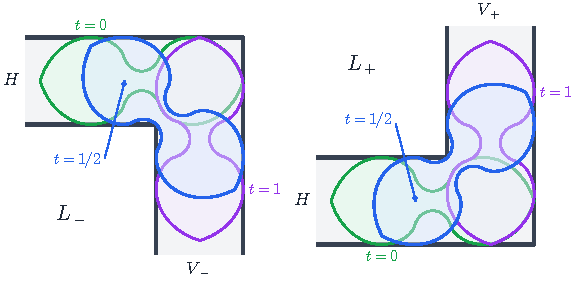
\includegraphics[width=\textwidth]{figures/fig-intro.pdf}
 \caption{Romik's sofa passing a right-turning corner (left) and a
 left-turning corner (right), from the same placement in the incoming
 arm. The illustrated motions turn through $-\pi/2$ and $\pi/2$,
 respectively.}\label{fig:intro}
\end{figure}

\subsection{Previous work}

Hammersley gave an early construction and the upper bound $2\sqrt2$ for
the ordinary problem \cite{Hammersley68}. Gerver constructed a sofa of
area $2.2195\ldots$ in 1992 \cite{Gerver92}, and Baek proved its
optimality \cite{Baek}. Requiring passage through both corners gives
a different extremal problem. The ambidextrous variant appears in
accounts of geometric problems \cite{CroftFalconerGuy91,Stewart04};
Gibbs obtained a numerical shape of area approximately $1.64495$
\cite{Gibbs14} before Romik found its exact description.

Romik derived differential equations for the contacts between a sofa
and the hallway walls, and solved them for the ambidextrous construction
\cite[Theorem~5]{Romik18}. Its boundary is piecewise algebraic, and
its area can be expressed by radicals and an inverse tangent. The
equations describe the construction within its contact pattern; they
do not give an upper bound for all admissible shapes and motions.
Kallus and Romik developed computer-assisted upper bounds for the
moving sofa problem \cite{KallusRomik18}. O'Keefe gives upper bounds
for its ambidextrous variant \cite{OKeefe26}, and Georgiev,
G\'omez-Serrano, Tao and Wagner list the ambidextrous problem as
Problem~6.63 \cite{GGTW25}.

We use Baek's theorem only to bound the areas of two auxiliary
ordinary sofas that occur in strict exclusions. The form needed here
is the rational upper bound $2.2199$; \cref{app:ordinary-sofa}
states this input and explains why it applies to those bodies.

\subsection{The strategy of the optimality proof}\label{sec:strategy-optimality}

Place the incoming sofa in the strip
$\Strip=\R\times[0,1]$. Its convex hull determines two downward
convex caps, $U$ and $V$: the upper hull boundary is the roof of $U$,
and reflecting the lower hull boundary in the midline gives the roof
of $V$. Each passage cuts a niche out of that hull. We must bound the
exterior roof area left after paying for the middle niche. At a
maximum, moving a supporting wall balances those two areas; the balance
then constrains the boundary curvature. This gives the following steps.

\begin{enumerate}[label=(\arabic*)]
 \item \emph{Pass from the actual motions to two cap scores.}
 Unless $|S|\le\sqrt2$, each passage supplies an effective turning
 angle in $(\pi/4,\pi/2]$. Let these angles be $\alpha$ and $\gamma$.
 The intermediate value theorem supplies every intervening hallway
 frame, even if the passage reverses its rotation. For a cap with
 projection $I$ and middle half $J$, define
 \[
  P_\alpha(U)=\int_{I\setminus J}f_U
                    -\int_J N_\alpha(U).
 \]
 Here $f_U$ is its roof and $N_\alpha(U)$ is the lower barrier imposed
 by the turn. The score counts the roof over the exterior quarters
 and subtracts the barrier over the middle half. An exact partition
 of vertical fibers gives
 \[
  |S|\le P_\alpha(U)+P_\gamma(V)
  \qquad\text{(\cref{sec:reduction}).}
 \]
 \item \emph{Obtain geometric laws for every maximizing cap.}
 After a horizontal translation, competitive caps lie in a fixed
 rectangle, and the score is continuous under Hausdorff convergence.
 A maximizer therefore exists. Cutting its middle roof to the chord
 joining the two middle endpoints, then restoring height one,
 cannot decrease its score. We approximate each prescribed canonical
 maximizer by polygons selected with a penalty for moving away from
 it (\cref{sec:selection}). Moving one polygon side compares the
 exterior roof gained with the inner-wall region lost. Passing these
 inequalities to the prescribed limit gives curvature bounds and
 endpoint laws (\cref{sec:variations}).
 \item \emph{Classify the full-turn maximizers.}
 The variation laws first exclude a tilted middle chord and force the
 middle roof to be horizontal (\cref{sec:full-turn}). They then give
 enough control of the two boundary arcs to identify the cap score
 with a functional of its support coordinates. A strict quadratic
 estimate and the equations of its stationary profiles show that
 this functional is at most $\Mc/2$, with equality only at Romik's
 support profile (\cref{sec:calibration}).
 \item \emph{Exclude equality at every proper turning angle.}
 If $\alpha<\pi/2$, the final outgoing strip imposes its first inner
 wall over the whole projection. This wall is part of $N_\alpha$,
 even where it rises above the swept niche. A variation bounds the
 length of the middle interval where this terminal wall is exposed.
 A weighted estimate for the opposite boundary arc forces that
 exposed interval to be longer, giving a contradiction
 (\cref{sec:partial-turn}). Thus $P_\alpha(U)\le\Mc/2$ for all
 angles under consideration, and equality requires a full turn.
\end{enumerate}

The small-area alternative satisfies $\sqrt2<\Mc$. In the other
case, steps (1), (3), and (4) give
\begin{equation}\label{eq:proof-chain}
 |S|\le P_\alpha(U)+P_\gamma(V)
     \le\frac\Mc2+\frac\Mc2=\Mc.
\end{equation}
The construction and exact area calculation in \cref{app:romik}
show that the upper bound is attained.

\subsection{The strategy of the uniqueness proof}\label{sec:strategy-uniqueness}

Suppose $|S|=\Mc$. Each inequality in \eqref{eq:proof-chain} is
then an equality. It follows that both original caps maximize their
scores. To identify $S$, the cap classification must apply to these
particular caps. The existence of a favorable maximizer would not
suffice: selecting a different maximizer, or replacing a middle roof
by its chord, can lose the information about the body that produced it.

This is why step (2) uses a penalty to select a prescribed cap. The
variation laws hold for every canonical maximizer, so the strict
support-function estimate identifies each one. The equality terms in
the chord cut and height restoration then recover the cap before
those operations. For a proper angle, the terminal-wall contradiction
is likewise applied to the prescribed maximizing pair $(\alpha,U)$.
Consequently equality in a cap score holds precisely when its angle
is $\pi/2$ and its cap is a horizontal translate of $\KR$.

The two caps of $S$ have the same projection. Their translates of
$\KR$ therefore align, and their intersection, after reflecting the
second cap, is a translate of Romik's hull. The original passage
constraints put $S$ inside the corresponding translate of $\SR$.
Equal area first gives equality up to a null set. Since $S$ is closed
and $\SR$ is the closure of its interior, a missing point would leave
a nonempty open subset of the interior missing as well, of positive
area. Thus the two compact sets are equal
(\cref{sec:equality,sec:recovery}). Applying this argument to any
witnessing pair of motions also forces each of its effective angles
to be $\pi/2$, proving the angular conclusion of \cref{thm:main}.

\subsection{Organization}

\Cref{sec:setting} defines the hallways, passages, caps, and scores.
\Cref{sec:reduction} proves the reduction from the two actual motions.
\Cref{sec:selection,sec:variations} obtain the approximation and
variation laws used by the analytic proof. \Cref{sec:full-turn,sec:calibration}
classify full-turn maximizers, and \cref{sec:partial-turn} proves the
universal cap bound and its strictness at proper angles.
\Cref{sec:equality} proves optimality and determines both equality
caps; \cref{sec:recovery} recovers the original compact body and proves
the quarter-turn conclusion. \Cref{sec:questions} gives further questions.

\Cref{app:ordinary-sofa} records the ordinary-sofa result used in
two exclusions. \Cref{app:romik} describes Romik's sofa, proves its
two explicit passages, and calculates its exact area.
\Cref{app:full-turn-estimates} proves the support-integral identities
and contact-energy estimates used for a full turn;
\cref{sec:variation-estimates} supplies the low-height exclusion.
\Cref{app:partial-turn-estimates} contains the initial-angle, circle,
and reflected-support estimates for the terminal tail.
\Cref{app:horizontal-estimates} gives the width and curvature estimates
for a horizontal middle, and \cref{app:preliminary-estimates} gives
the preliminary width and tilt bounds. Finally,
\cref{app:tilted-selector} excludes the remaining tilted configurations.
